% LTeX: language=pl-PL
\chapter{Mechanika kwantowa}
\chapterauthor{PG}
% +Oskar Słowik w wydaniu 2

Mechanika kwantowa opisuje zachowania bardzo małych cząstek fizycznych,
czyli~np.~fotonów, elektronów albo~kwantowych bitów -- kubitów.
Na~potrzeby niniejszej~książki przyjmiemy, że~nie~będą nas interesować
ich właściwości fizyczne, a~tylko pewne abstrakcyjne stany,
w~jakich~mogą~się znajdować. Stany te numerujemy zazwyczaj przy~użyciu
liczb naturalnych: 0, 1, 2 itd. Stany kwantowe opisują np. polaryzację
fotonu, energię elektronu na~orbicie atomu, drgania sieci krystalicznej,
spin cząstki lub~jeszcze~inne właściwości układów kwantowych.

Informatyków często nie~interesuje, w~jaki~sposób właściwości fizyczne układów
są~wykorzystywane do~zapisu informacji klasycznej w~komputerze klasycznym --
a~zauważmy, że~do~tego~celu może zostać wykorzystana magnetyzacja powierzchni na
talerzu dysku twardego, napięcie elektryczne w~obwodzie wewnątrz procesora czy~wartość
natężenia prądu w~przewodzie elektrycznym. Dlatego też informatyków kwantowych nie~musi
interesować to, w~jaki sposób informacja kwantowa jest fizycznie zapisana
w~komputerze kwantowym.

Gdy~mówimy o~mechanice kwantowej, a~zatem również~o~informatyce kwantowej, posługujemy~się
fizycznym pojęciem \emph{doświadczenia}. Doświadczenie -- w~znaczeniu, jakie~będziemy
nadawać mu w~niniejszym tekście -- składa~się z~trzech etapów:
\begin{itemize}
	\item przygotowania,
	\item ewolucji,
	\item pomiaru i~interpretacji wyników.
\end{itemize}

W~interesującym nas~kontekście możemy opisać poszczególne etapy doświadczenia
następująco: przygotowujemy stan kwantowy, przeprowadzamy ewolucję kwantową
tego~stanu i -- na~koniec -- wykonujemy pomiar kwantowy (patrz:
Rysunek~\ref{rys:doswiadczenie}).
\begin{figure}[t]
	\centering
	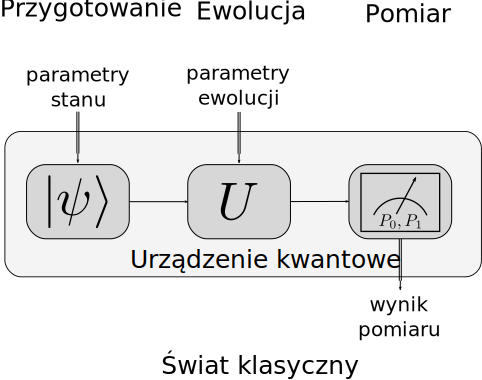
\includegraphics[width=0.7\textwidth]{pics/eksperymentkwantowy}
	\caption{Schematyczna reprezentacja doświadczenia kwantowego}
	\label{rys:doswiadczenie}
\end{figure}

Zauważmy, że~w~podobny sposób wykonujemy w~informatyce obliczenia klasyczne:
przygotowujemy dane (stan początkowy); następnie wykonujemy program (ewolucja)
i~odczytujemy wynik (pomiar). Współczesne komputery wykonują te~trzy etapy jako~przeprowadzane
nieustannie obliczenia. Nie~obserwujemy tych etapów podczas~codziennych
interakcji z~komputerem, więc nie~zauważamy w~sposób świadomy powyższego schematu
działania.

Każde urządzenie informatyczne działające na~podstawie zasad informatyki
kwantowej -- lub,~w~skrócie,
komputer kwantowy -- musi być wyposażone zarówno w~podukład kwantowy,
jak~i~podukład klasyczny, czyli~jakąś~formę komputera klasycznego,
np.~elektronicznego.
Komputer klasyczny będzie w~takim urządzeniu odpowiadał za~sterowanie układem
kwantowym, komunikację ze~światem zewnętrznym oraz~interpretację wyników
działania komputera kwantowego. Schemat konstrukcji i~działania komputera
kwantowego sprzężonego z~komputerem klasycznym
przedstawiono na~Rysunku~\ref{rys:komputer}.
\begin{figure}
	\centering
	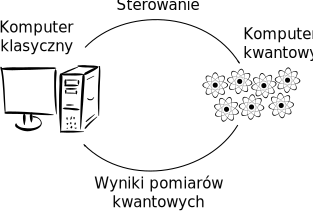
\includegraphics[width=0.7\textwidth]{pics/sterowaniepomiar}
	\caption{Schematyczna reprezentacja działania kwantowego urządzenia informatycznego. Komputer klasyczny steruje
		komputerem kwantowym, komputer kwantowy zwraca wyniki pomiarów do komputera klasycznego.}
	\label{rys:komputer}
	% https://openclipart.org/detail/15831/stylized-atom
	% https://openclipart.org/detail/1953/minimalist-monitor-and-computer
\end{figure}

W~przypadku bardziej~złożonym -- kiedy~chcemy opisać sieć komputerów kwantowych
i~jej wykorzystanie -- mówimy zazwyczaj również~o~użytkownikach tej sieci, którzy
mają do~dyspozycji komputery kwantowe i~klasyczne oraz~kwantowe i~klasyczne
połączenia sieciowe. Na~potrzeby opisu w~literaturze przedmiotu nadaje im~się umowne imiona:
,,Alicja'' (użytkownik A), ,,Bob'' (użytkownik B) oraz~,,Ewa'' (podsłuchujący)%
\footnote{Po~angielsku -- ,,Alice'', ,,Bob'' i~,,Eve''. Imiona ,,Alice'' i~,,Bob'' są używane, ponieważ~można
	je oznaczyć literami A i~B, natomiast~,,Eve'' pochodzi od~angielskiego słowa \emph{eavesdropping} -- czyli~podsłuchiwanie.}.
Pierwsze dwie osoby próbują się~komunikować, a~ostatnia próbuje im w~tym przeszkodzić.
Nietrudno zauważyć, że~w~komiksie dość~swobodnie nawiązujemy do~tej konwencji.

\section{Formalizm matematyczny}
Mechanika kwantowa jest opisywana przy~pomocy formalizmu (czyli języka)
matematycznego, który wykorzystuje liczby zespolone, wektory oraz~macierze.
Bez~jego zrozumienia nie~jest zatem możliwe zrozumienie samej mechaniki
kwantowej. Jednakże~w~niniejszej książce najpierw skupimy~się na~przedstawieniu
pojęć ściśle związanych z~mechaniką i~informatyką kwantową, natomiast~opis
formalizmu matematycznego znajdziesz w~rozdziale~\ref{ch:podstawy} zamieszczonym na~końcu.
Uznaliśmy~bowiem, że~nie~chcemy Cię zmuszać do~nauki materiału
matematycznego, skoro jeszcze nie~znasz powodów, dla~których opanowanie tego
formalizmu jest Ci~niezbędne. Oczywiście możesz zacząć od~lektury rozdziału~\ref{ch:podstawy} --
a~jeśli~się~na~nią nie~zdecydujesz, zachęcamy do~zerkania do~niego, ilekroć
nie~będziesz rozumieć jakiegoś pojęcia lub~symbolu matematycznego.

\section{Kubit}
Elementarnym obiektem w~informatyce kwantowej jest \newterm{kubit}\index{kubit},
który jest najprostszym układem kwantowym. Stan kubitu (zdefiniowany poniżej) opisuje wektor o~dwóch
elementach zespolonych.

W~celu opisania stanu kubitu zwyczajowo wybieramy bazę obliczeniową
$$
	\ket{0}=\begin{bmatrix} 1\\ 0\end{bmatrix},
	\ket{1}=\begin{bmatrix} 0\\ 1\end{bmatrix}.
$$
Wówczas dowolny stan $\ket{\psi}$ kubitu tworzy liniową kombinację wektorów bazowych
$$
	\ket{\psi}=\alpha\ket{0}+\beta\ket{1},
	\label{equ:kubit}
$$ z~$|\alpha|^2+|\beta|^2=1$ oraz $\alpha, \beta \in
	\Complex$.

Liczby $\alpha$ i~$\beta$ są zespolone, zatem aby~je zapisać, potrzebujemy
czterech liczb rzeczywistych. Jednak~ponieważ zachodzi warunek $|\alpha|^2+|\beta|^2=1$,
jedną z~potrzebnych nam liczb możemy wyliczyć z~pozostałych trzech. Wynika z~tego,
że~dowolny stan kubitu może być opisany przez~trzy liczby rzeczywiste.
Taki przykładowy opis jest zadany równaniem
$$
	\ket{\psi}=e^{\i\gamma}\left(
	\cos{\frac{\theta}{2}}\ket{0}+e^{\i\phi}\sin{\frac{\theta}{2}}\ket{1}
	\right),
$$
gdzie~$\gamma, \theta, \phi\in\mathbb{R}$.
Współczynnik $e^{\i\gamma}$ nazywamy \newterm{fazą globalną}\index{faza
	globalna}. Jak~się~później przekonamy, nie~ma on większego znaczenia, więc~zawsze
możemy przyjmować, że~równa~się on 1, czyli~$\gamma=0$. Zatem w~efekcie
dostajemy taką~oto~postać wzoru stanu kubitu:
$$
	\ket{\psi}=
	\cos{\frac{\theta}{2}}\ket{0}+e^{\i\phi}\sin{\frac{\theta}{2}}\ket{1}.
$$

Jeżeli dwa stany różnią~się fazą globalną, to fizycznie te stany są takie
same. Zatem każdy stan możemy również pomnożyć przez~dowolną liczbę w~postaci
$e^{\i\gamma}$, nie~zmieniając tego stanu.

Liczby rzeczywiste $\theta$ i~$\phi$ mogą być interpretowane jako~współrzędne
punktu na~trójwymiarowej sferze o~promieniu 1. Sferę taką~nazywamy
\emph{sferą Blocha}\index{sfera Blocha}. Będziemy ją bardzo często wykorzystywać
do~wizualizacji operacji na~kubicie.

\subsection{Sfera Blocha}
\begin{figure}[h]
	\begin{center}
		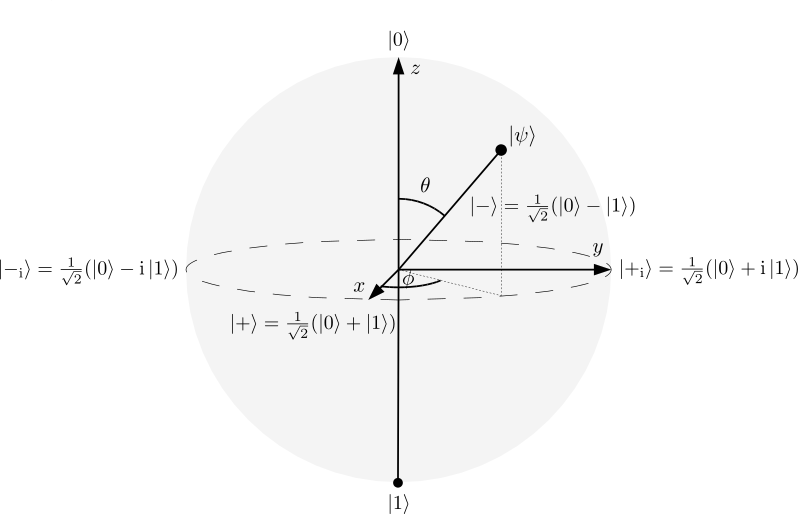
\includegraphics[width=0.8\textwidth]{pics/bloch}
	\end{center}
	\caption{Sfera Blocha}
	\label{rys:sferablocha}
\end{figure}
Sfera Blocha\footnote{Od nazwiska szwajcarskiego fizyka Feliksa Blocha
	(1905 -- 1983).} (Rysunek~\ref{rys:sferablocha}) jest wygodną
reprezentacją graficzną kubitu. Na powierzchni sfery Blocha znajdują się
punkty odpowiadające stanom kwantowym. Zazwyczaj rysujemy ją
w~taki~sposób, że~stan $\ket{0}$ oznaczamy u~góry, stan $\ket{1}$
u~dołu,
$\ket{-_\i}=\frac{1}{\sqrt{2}} (\ket{0}-\i\ket{1})$ po~lewej stronie,
$\ket{+_\i}=\frac{1}{\sqrt{2}}
	(\ket{0}+\i\ket{1})$ -- po~prawej, $\ket{+}=\frac{1}{\sqrt{2}} (\ket{0}+\ket{1})$ z~przodu,
a~$\ket{-}=\frac{1}{\sqrt{2}} (\ket{0}-\ket{1})$ z~tyłu.

W~dalszej części tekstu zostanie opisane, w~jaki~sposób bramki kwantowe działają
na~kubit -- a~odwzorowania zostaną zaprezentowane właśnie na~sferze Blocha.

\section{Stan}
\emph{Stanem}\index{stan!kwantowy} w~mechanice kwantowej nazywamy wektor
$$
	\ket{\psi}=
	\begin{bmatrix}
		\alpha_0 \\
		\alpha_1 \\
		\vdots   \\
		\alpha_{n-1}
	\end{bmatrix},
$$
który możemy zapisać również w~bazie obliczeniowej w~postaci
$$
	\ket{\psi}=\alpha_0\ket{0} + \alpha_1 \ket{1} + \ldots + \alpha_{n-1} \ket{n-1}.
$$
Chcemy, aby~$\alpha_i \in \Complex$ dla~$i=0, 1, \ldots, n-1$, tzn.~współczynniki
wektora, były liczbami zespolonymi, oraz~aby~$\norm{\ket{\psi}} = \sqrt{\abs{\alpha_0}^2
		+ \abs{\alpha_1}^2 + \ldots + \abs{\alpha_{n-1}}^2} = 1$, tzn.~aby~norma
euklidesowa wektora\index{wektor!norma euklidesowa} wynosiła
1\footnote{Zauważ, że baza obliczeniowa jest ortonormalna\index{baza
		ortonormalna}.}.

Liczby $\alpha_i \in \Complex$ nazywamy
\emph{amplitudami prawdopodobieństwa}\index{amplituda prawdopodobieństwa} stanu kwantowego. Gdy~jedna
z~tych liczb jest równa 1, możemy powiedzieć -- nieformalnie -- że~układ
kwantowy jest w~stanie odpowiadającym tej liczbie. Na~przykład jeżeli~$\alpha_0=1$,
mówimy, że~układ kwantowy jest w~stanie $\ket{0}$.

Jeżeli żadna z~liczb $\alpha_i$ nie~jest równa 1, to~znaczy, że~przynajmniej dwie
amplitudy prawdopodobieństwa są niezerowe. Wówczas mówimy, że~układ jest w~\emph{superpozycji}
stanów\index{superpozycja}. Przykładowo: jeżeli mamy układ z~$n=3$ i~$\alpha_0 = \alpha_2 = 1/\sqrt{2}$, tzn.~nasz
stan zapisujemy jako~$1/\sqrt{2}\ket{0}+1/\sqrt{2}\ket{2}$, to~mówimy, że~stan
jest w~superpozycji stanu $\ket{0}$ oraz~$\ket{2}$.

\section{Stany wielosystemowe}
\subsection{Dwa kubity}
Operacją matematyczną, która~odpowiada złączeniu układów dwóch kubitów, jest
\newterm{iloczyn Kroneckera}\footnote{Od nazwiska niemieckiego matematyka Leopolda Kroneckera (1823 -- 1891).}\index{iloczyn Kroneckera}.
Jeśli dane są stany dwóch kubitów $\ket{\psi}$ i~$\ket{\phi}$:
$$
	\ket{\psi}=
	\begin{bmatrix}
		\alpha \\
		\beta
	\end{bmatrix}
	=\alpha\ket{0}+\beta\ket{1}
	,
	\ket{\phi}=
	\begin{bmatrix}
		\gamma \\
		\delta
	\end{bmatrix}
	= \gamma\ket{0}+ \delta\ket{1},
$$
to ich~łączny stan zapisujemy następująco:
$$
	\ket{\psi}\otimes\ket{\phi}=
	\begin{bmatrix}
		\alpha \gamma \\
		\alpha \delta \\
		\beta \gamma  \\
		\beta \delta
	\end{bmatrix}=
	\alpha \gamma\ket{0}\otimes\ket{0}+
	\alpha \delta\ket{0}\otimes\ket{1}+
	\beta \gamma\ket{1}\otimes\ket{0}+
	\beta \delta\ket{1}\otimes\ket{1},
$$
bądź~w~skrócie:
$$
	\ket{\psi\phi}=
	\alpha \gamma\ket{00}+
	\alpha \delta\ket{01}+
	\beta \gamma\ket{10}+
	\beta \delta\ket{11}.
$$

Jak~widać, etykiety $00$, $01$, $10$ oraz~$11$ odpowiadają liczbom $0$, $1$, $2$
oraz~$3$ zapisanym binarnie.
Zatem stan $\ket{\psi\phi}$ możemy zapisać jako:
$$
	\ket{\psi\phi} =
	\alpha \gamma\ket{0}+
	\alpha \delta\ket{1}+
	\beta \gamma\ket{2}+
	\beta \delta\ket{3}.
$$
Zapiszmy teraz nowy stan:
$$
	\ket{\Phi} = c_0\ket{0} + c_1\ket{1} + c_2\ket{2} + c_3\ket{3}
$$
i~zastanówmy się, czy~istnieją takie~liczby $c_0, c_1, c_2, c_3$,
dla~których nie~da~się znaleźć takich~$\alpha, \beta, \gamma, \delta$,
które spełniają układ równań $$c_0=\alpha \gamma,\; c_1=\alpha \delta,\; c_2=\beta \gamma,
	\text{ oraz } c_3=\beta \delta.$$

Weźmy pod~uwagę stan $\ket{\Phi^+}=\frac{1}{\sqrt{2}}(\ket{0}+\ket{3})$
i~dla~uproszczenia opuśćmy czynnik $\frac{1}{\sqrt{2}}$. Wtedy~mamy
$c_0=c_3=1$ oraz~$c_1=c_2=0$. Załóżmy, że~nasz stan możemy zapisać w~postaci
$\alpha \gamma\ket{0}+ \alpha \delta\ket{1}+\beta
	\gamma\ket{2}+\beta \delta\ket{3}$. Wówczas uzyskujemy układ równań:
$$\alpha \gamma=1,\; \alpha \delta=0,\; \beta\gamma=0,\; \beta\delta=1.$$
Zauważmy, że~$\alpha,
	\beta, \gamma, \delta \geq 0$, co~wynika z~tego, że~$|\alpha|^2+|\beta|^2 = 1$
oraz~$|\delta|^2+|\gamma|^2 = 1$. Zatem aby~spełnić pierwszy warunek $\alpha = \gamma = 1$,
natomiast aby~spełnić drugi warunek $\delta = 0$.
Jednakże~z~czwartego warunku wynika, że~$\delta = 1$. Zatem otrzymujemy
sprzeczność. Wnioskujemy z~tego, że~stanu $\ket{\Phi^+}$ nie~da~się zapisać jako iloczynu
Kroneckera dwóch stanów. Stan $\ket{\Phi^+}$ nazywamy \newterm{stanem
	Bella}\index{stan!Bella}\footnote{Od~nazwiska brytyjskiego fizyka Johna S.~Bella (1928 -- 1990).}. Ma on
wyjątkowo istotne znaczenie w~informatyce kwantowej.

\subsection{Wiele układów kwantowych}
Gdy~mamy do~dyspozycji $n$ kubitów w~stanach
$$\ket{\psi_1}, \ket{\psi_2}, \ldots, \ket{\psi_n},$$
wówczas~możemy opisać je jako~jeden łączny układ, którego~stan ma
$2^n$ współczynników. Operacją matematyczną,
która w~sposób zbiorczy opisuje takie~połączenie wielu kubitów, jest
iloczyn Kroneckera. Jeżeli~kubity nie~są ze~sobą związane (splątane), to stan
takiego układu jest opisany przez~łączny stan
$$
	\ket{\Psi}=\ket{\psi_1}\otimes \ket{\psi_2}\otimes \ldots\otimes \ket{\psi_n}.
$$

\subsection{Splątanie kwantowe}
Splątanie kwantowe jest zjawiskiem, które dotyczy tylko~i~wyłącznie obiektów
podlegających prawom mechaniki kwantowej. Splątane mogą być dwa układy (lub~więcej), które miały okazję ze~sobą
oddziaływać w~przeszłości. Matematycznie definicja
splątania dwóch układów jest następująca: jeżeli~danego stanu $\ket{\phi}$,
który opisuje stan dwóch układów, nie~możemy
zapisać jako~$\ket{\psi_1}\otimes\ket{\psi_2}$ dla~jakichkolwiek $\ket{\psi_1}$
oraz~$\ket{\psi_2}$, to jest on \newterm{splątany}\index{stan!splątany}. Jeżeli~natomiast
istnieją takie $\ket{\psi_1}$ oraz~$\ket{\psi_2}$, że~$\ket{\phi}=\ket{\psi_1} \otimes \ket{\psi_2}$, to stan nazywamy
\newterm{separowalnym}\index{stan!separowalny}.
Jak widać, wspomniany wcześniej stan Bella $\ket{\Phi^+}$ jest stanem
splątanym.

Splątanie wielu układów kwantowych\index{stan!splątany!wiele układów kwantowych} jest problemem znacznie bardziej~złożonym. Jeżeli~mamy
np.~trzy układy, to pierwsze dwa mogą być splątane ze~sobą, ale~nie~z~trzecim,
jak~na~przykład w~stanie
$$
	\frac{1}{\sqrt{2}}(\ket{00}+\ket{11})\otimes \ket{1}.
$$
Wszystkie trzy układy mogą być ze~sobą splątane na~różne sposoby. Przykładowo stany
$$
	\ket{W}=\frac{1}{\sqrt{3}}(\ket{001}+\ket{010}+\ket{100})
$$
oraz
$$
	\ket{GHZ}=\frac{1}{\sqrt{2}}(\ket{000}+\ket{111})
$$
są splątane w~całkowicie różny sposób -- przy~czym~wytłumaczenie tego faktu wykracza poza~zakres tej książki.

Stany splątane mają bardzo nieintuicyjne właściwości. Na przykład,
jeżeli cząstki będące w~stanie splątanym oddalimy bardzo daleko
od~siebie, pozostaną one ze~sobą związane. Będziemy mieli okazję
zaobserwować ten efekt, gdy~będzie mowa o~pomiarze stanów splątanych.

\section{Ewolucja kwantowa}
\newterm{Ewolucja kwantowa}\index{ewolucja kwantowa}
to nazwa, którą opisujemy zmianę stanu kwantowego w~czasie. Zakładamy, że~mamy
pewien stan w~chwili $0$, a~dzięki ewolucji kwantowej uzyskujemy stan w~chwili $1$.
Zwróćmy tutaj uwagę na~pewien fakt dotyczący stanów kwantowych: norma stanu kwantowego wynosi zawsze 1.
Normę tę utożsamiamy z~prawdopodobieństwem całkowitym. Zatem jeżeli~chcemy, by~prawdopodobieństwo
całkowite było zachowane, oznacza to, że~chcemy, by matematyczny opis
ewolucji zachowywał normę wektora stanu. Norma wektora jest zachowywana
wyłącznie przez~obroty i~symetrie. Taki opis matematyczny ewolucji możemy uzyskać z wykorzystaniem macierzy
unitarnych. Dla~uproszczenia opisu pomijamy tutaj kwestię wymiarów macierzy
i~wektorów stanów. Oczywiście wymiary muszą być tak dobrane, by można było
mnożyć odpowiadające sobie~nawzajem wymiarami macierze i~wektory.

Przejście ze~stanu w~chwili $0$ $\ket{\psi_{t=0}}$ do~stanu w~chwili
$1$ $\ket{\psi_{t=1}}$ jest zadane przez
$
	\ket{\psi_{t=1}}= \mat{U}\ket{\psi_{t=0}},
$
gdzie~$\mat{U}$ jest macierzą unitarną.

Powyższe, pozornie trywialne, równanie opisuje zachowanie wszystkich układów kwantowomechanicznych, w~tym oczywiście
komputerów kwantowych. W~informatyce kwantowej macierze unitarne\index{macierz!unitarna} przeważnie
nazywamy \newterm{bramkami kwantowymi}\index{bramka!kwantowa}.

Zauważmy od~razu pewną charakterystyczną cechę mechaniki kwantowej, wynikającą z~powyższego
równania: pamiętając, że~macierz odwrotna $\mat{U}^{-1}$ do~macierzy
unitarnej zawsze istnieje i~jest jej sprzężeniem hermitowskim $\mat{U}^\dagger$,
możemy zapisać to równanie odwrócone w~czasie:
$
	\ket{\psi_{t=0}}= \mat{U}^\dagger\ket{\psi_{t=1}}.
$
Dlatego~też~mówimy, że~ewolucja kwantowa jest \emph{odwracalna w~czasie}.

\section{Bramki kwantowe}
Bramek kwantowych jest nieskończenie wiele -- jednakże~my, mimo~ich mnogości,
skupimy~się tylko na~bramkach działających na~jeden lub~dwa kubity. Bramki te
wystarczają do~tego, by zbudować dowolny komputer kwantowy lub~kwantowe
urządzenie komunikacyjne. Są one zatem najciekawsze z~punktu widzenia
informatyka kwantowego.

\subsection{Bramki jednokubitowe}
Dla~jednego kubitu możemy zapisać wiele różnych bramek kwantowych\index{bramka!jednokubitowa}.
Na~początek zdefiniujmy bramkę obrotu wokół osi~$y$ o~kąt~$\gamma$:
$$
	\mat{R_y}(\gamma)=
	\begin{bmatrix}
		\cos({\frac{\gamma}{2}})  & \sin({\frac{\gamma}{2}}) \\
		-\sin({\frac{\gamma}{2}}) & \cos({\frac{\gamma}{2}})
	\end{bmatrix},
$$
bramkę obrotu wokół osi~$z$ o~kąt~$\beta$:
$$
	\mat{R_z}(\beta)=
	\begin{bmatrix}
		e^{\frac{\i\beta}{2}} & 0                      \\
		0                     & e^{\frac{-\i\beta}{2}}
	\end{bmatrix}
$$
oraz~bramkę zmieniającą fazę globalną o~czynnik~$\alpha$:
$$
	\mat{Ph(\alpha)}=
	\begin{bmatrix}
		e^{\i\alpha} & 0            \\
		0            & e^{\i\alpha}
	\end{bmatrix}.
$$
Działanie bramek $\mat{R_z}(\beta)$ oraz~$\mat{R_y}(\gamma)$ zostało pokazane na~Rysunku \ref{rys:bramki-obrotów}.
Bramka $\mat{Ph(\alpha)}$ zmienia tylko globalną fazę, zatem jej działania nie~można zaobserwować na~sferze Blocha.

Dowolna bramka działająca na~jednym kubicie może zostać zapisana jako złożenie
czterech bramek: zmiany fazy oraz trzech obrotów, w~postaci
opisanej przez~cztery liczby rzeczywiste $\alpha, \beta, \gamma, \delta$:
\begin{equation*}
	\begin{split}
		\mat{U}(\alpha, \beta, \gamma, \delta)=&
		\mat{Ph}(\alpha)\mat{R_z}(\beta)\mat{R_y}(\gamma)\mat{R_z}(\delta)
		=\\
		=&
		\begin{bmatrix}
			e^{\i\alpha} & 0            \\
			0            & e^{\i\alpha}
		\end{bmatrix}
		\begin{bmatrix}
			e^{\frac{\i\beta}{2}} & 0                      \\
			0                     & e^{\frac{-\i\beta}{2}}
		\end{bmatrix}
		\begin{bmatrix}
			\cos({\frac{\gamma}{2}})  & \sin({\frac{\gamma}{2}}) \\
			-\sin({\frac{\gamma}{2}}) & \cos({\frac{\gamma}{2}})
		\end{bmatrix}
		\begin{bmatrix}
			e^{\frac{\i\delta}{2}} & 0                       \\
			0                      & e^{\frac{-\i\delta}{2}}
		\end{bmatrix}
		.
	\end{split}
\end{equation*}
Pierwszy obrót to obrót wokół osi~$z$, drugi -- wokół osi~$y$, a~trzeci -- ponownie wokół $z$.

\begin{figure}
	\centering
	\subbottom[Bramka $\mat{R_z}(\beta)$ dokonująca obrotu wokół osi $z$ łączącej $\ket{0}$ z~$\ket{1}$.
		\label{rys:bramka-rz}]{\includegraphics[width=0.46\linewidth]{pics/Rz}}
	\hfill
	\subbottom[Bramka $\mat{R_y}(\gamma)$ dokonująca obrotu wokół osi $y$ łączącej $\ket{+_\i}$
		z~$\ket{-_\i}$.\label{rys:bramka-ry}]{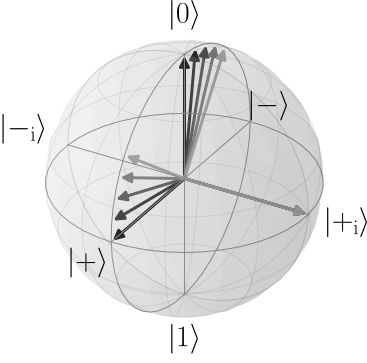
\includegraphics[width=0.46\linewidth]{pics/Ry}}
	\caption{Działanie bramek $\mat{R_z}(\beta)$ -- panel~\subcaptionref{rys:bramka-rz} oraz~$\mat{R_y}(\gamma)$
	-- panel~\subcaptionref{rys:bramka-ry} na~stanach $\ket{0}$, $\ket{+}$, $\ket{+_\i}$ (czarne strzałki).
	Wartości $\beta$ oraz~$\gamma$ rosną zgodnie z~przechodzeniem kolorów strzałek od~ciemniejszych
	do~jaśniejszych i~wynoszą $(0{,}05\pi,0{,}1\pi,0{,}15\pi,0{,}2\pi)$.
	}
	\label{rys:bramki-obrotów}
\end{figure}

Bramki kwantowe mają swoje oznaczenia graficzne. Bramkę
je\-dno\-ku\-bi\-to\-wą oznacza~się jako prostokąt, wewnątrz~którego zapisana jest nazwa
bramki. Przykład takiej bramki kwantowej pokazano na~Rysunku~\ref{rys:bramkakubitowa}.
\begin{figure}[h]
	\begin{center}
		\begin{minipage}{4in}
			\centering
			\Qcircuit @C=1em @R=.7em {
			\lstick{\ket{\psi}} & \gate{\mat{U}}  &  \rstick{\mat{U}\ket{\psi}} \qw
			}
		\end{minipage}
	\end{center}
	\caption{Rysunek przedstawiający bramkę jednokubitową $\mat{U}$. Pojedyncza
		linia przechodząca przez~bramkę oznacza kubit. Stan wejściowy do~bramki --
		po~lewej stronie, wyjściowy -- po~prawej.}
	\label{rys:bramkakubitowa}
\end{figure}

\subsubsection{Bramki jednokubitowe}
Kilka spośród~wszystkich bramek kwantowych\index{bramka!jednokubitowa} ma swoje ustalone nazwy, które są
często wykorzystywane w~informatyce kwantowej. Poniżej prezentujemy ich przegląd,
zawierający informację o~tym, jak~wygląda macierz danej bramki, jak działa ona
na~ogólny stan $\ket{\psi}=\alpha\ket{0} + \beta\ket{1}$, a~także
interpretację jej działania na~sferze Blocha.

\newterm{Bramka identyczność}\index{bramka!identyczność} nie~zmienia stanu kubitu.
Oznaczamy ją przez~$\mat{\id}$. Jej~macierz zawiera jedynki na~diagonali i~zera poza~diagonalą:
$$\mat{\id}=\begin{bmatrix} 1 & 0 \\ 0 & 1\end{bmatrix}.$$
Działanie identycznością na~stan jest trywialne:
$$\mat{\id}(\alpha\ket{0} + \beta\ket{1}) = \alpha\ket{0} + \beta\ket{1}.$$

\newterm{Bramka negacji bitu}\index{bramka!negacji bitu}
oznaczana jest przez~$\mat{X}$. Jej macierz jest następująca:
$$\mat{X}=\begin{bmatrix} 0 & 1 \\ 1 & 0\end{bmatrix},$$
a~działanie polega na~zamianie stanu $\ket{0}$ na~$\ket{1}$
i~odwrotnie. Zatem gdy~te stany bazy obliczeniowej są w~superpozycji,
bramka~$\mat{X}$ zamienia pomiędzy~nimi amplitudy prawdopodobieństwa:
$$\mat{X} (\alpha\ket{0} + \beta\ket{1}) = \alpha\ket{1} + \beta\ket{0}.$$

\newterm{Bramka negacji fazy}\index{bramka!negacji fazy}, oznaczana przez~$\mat{Y}$,
ma następującą postać macierzową:
$$\mat{Y} = \begin{bmatrix} 0&-\i\\ \i&0 \end{bmatrix}.$$
Jej działanie polega na~wzajemnej zamianie stanów $\ket{+}$ oraz~$\ket{-}$.
Jej działanie na~superpozycję stanów bazy obliczeniowej jest następujące:
$$\mat{Y} (\alpha\ket{0} + \beta\ket{1}) = \alpha\i\ket{1} - \beta\i \ket{0},$$
ale~ponieważ możemy pomnożyć ten stan przez~fazę globalną $\i=e^{\frac{\i \pi}{2}}$, nie~zmieniając
stanu, to otrzymujemy $\beta\ket{0}-\alpha\ket{1}$.

\newterm{Bramka negacji fazy i~bitu}\index{bramka!negacji fazy i~bitu} oznaczana jest przez~$\mat{Z}$,
a~jej macierz jest następująca:
$$\mat{Z} = \begin{bmatrix} 1 & 0 \\ 0 & -1\end{bmatrix}.$$
Bramka ta zamienia ze~sobą stany $\ket{+_\i}$ oraz~$\ket{-_\i}$.
Jej działanie na~superpozycji wektorów bazy obliczeniowej jest następujące:
$$\mat{Z} (\alpha\ket{0} + \beta\ket{1}) = \alpha\ket{0} - \beta\ket{1}.$$
Zauważmy, że~bramki $\mat{X}$, $\mat{Y}$ oraz~$\mat{Z}$ mają ciekawą własność:
$$\mat{X}^2=\mat{Y}^2=\mat{Z}^2=\i\mat{X}\mat{Y}\mat{Z}=\mat{\id}.$$

\newterm{Bramki zmiany fazy}\index{bramka!zmiany fazy}
to rodzina bramek $\mat{R}(\phi)$ zależnych od~parametru rzeczywistego $\phi$.
Postać macierzowa tych bramek jest następująca:
$$\mat{R}(\phi) = \begin{bmatrix} 1 & 0 \\ 0 & e^{\i \phi} \end{bmatrix}.$$
Ich działanie zmienia fazę względną pomiędzy~stanami bazy obliczeniowej:
$$\mat{R}(\phi) (\alpha\ket{0} + \beta\ket{1}) = \alpha\ket{0} +  e^{\i \phi} \beta\ket{1}.$$
Działanie tej rodziny bramek przedstawia Rysunek~\ref{rys:bramka-Rphi}.

\begin{figure}[h]
	\centering
	\includegraphics[width=0.45\linewidth]{pics/Rphi}
	\caption{Wizualizacja działania bramek $\mat{R}(\phi)$ na~stanach
	$\ket{0}$, $\ket{+}$, $\ket{+_\i}$ (czarne strzałki).
	Wartości $\phi$ rosną w~miarę rozjaśniania~się kolorów strzałek i~wynoszą
	$(0{,}05\pi,0{,}1\pi,0{,}15\pi,0{,}2\pi)$.}
	\label{rys:bramka-Rphi}
\end{figure}

\newterm{Bramka Hadamarda}\footnote{Od nazwiska francuskiego matematyka
	Jacquesa Salomona Hadamarda (1865 -- 1963).}\index{bramka!Hadamarda}
jest
oznaczana symbolem $\mat{H}$, a~jej postać macierzowa jest następująca:
$$\mat{H}=\frac{1}{\sqrt{2}} \begin{bmatrix} 1 & 1 \\ 1 & -1\end{bmatrix}.$$
Bramka ta jest często pierwszym krokiem wielu algorytmów i~protokołów
kwantowych, gdyż~przeprowadza ona stany bazy obliczeniowej
do~ich superpozycji\index{superpozycja} w~następujący sposób:
$$
	\begin{aligned}
		\mat{H}\ket{0} = \frac{1}{\sqrt{2}}\left( \ket{0} +\ket{1} \right)=\ket{+}, \\
		\mat{H}\ket{1} = \frac{1}{\sqrt{2}}\left( \ket{0} -\ket{1} \right)=\ket{-}.
	\end{aligned}
$$

Zauważmy, że bramka Hadamarda jest odwrotnością samej siebie, tzn. że $\mat{H} = \mat{H}^{-1}$. Zatem
$$
	\begin{aligned}
		\mat{H} \ket{+} = \ket{0}, \\
		\mat{H} \ket{-} = \ket{1}.
	\end{aligned}
$$

Wiedząc, że macierz bramki Hadamarda jest unitarna, tzn. że
$\mat{H}^{-1}=\mat{H}^\dagger$, widzimy, że $\mat{H}=\mat{H}^\dagger$. A
to oznacza, że macierz bramki Hadamarda jest macierzą
hermitowską\index{macierz!hermitowska}.

\subsection{Bramki kontrolowane} W~przypadku bramek dwukubitowych możemy
stworzyć bramki kontrolowane. O~bramkach tych mówimy, że~jeden kubit
kontroluje bramkę, a~na~drugi nakładana jest dana bramka
$\mat{U}$. Bramka kontrolowana\index{bramka kwantowa!kontrolowana} ,,kontrolowane~$\mat{U}$'' działa
w~następujący sposób: jeżeli~kubit kontrolujący\index{kubit!kontrolujący} jest w~stanie $\ket{1}$, to nałóż
wybraną bramkę $\mat{U}$ na~kubit docelowy\index{kubit!docelowy};
jeżeli~kubit kontrolujący jest w~stanie $\ket{0}$, to nie~rób nic.

Bramkę taką możemy zapisać w~postaci
$$
	\mat{C}\mat{U}_1^2=\ketbra{0}{0}\otimes \mat{\id} + \ketbra{1}{1}\otimes \mat{U},
$$
gdzie indeks dolny oznacza numer kubitu kontrolującego, a~górny kontrolowanego.
Jeżeli~bramka $\mat{U}$ ma postać macierzową
$$
	\mat{U}=
	\begin{bmatrix}
		u_{00} & u_{01} \\
		u_{10} & u_{11}
	\end{bmatrix},
$$
to kontrolowana bramka $\mat{U}$ ma postać
$$
	\mat{C}\mat{U}_1^2 = \begin{bmatrix} 1 & 0 & 0 & 0 \\ 0 & 1 & 0 & 0 \\ 0 & 0 & u_{00} & u_{01} \\ 0 & 0 & u_{10} & u_{11}  \end{bmatrix},
$$
a jej działanie można zapisać jako:
\begin{eqnarray}
	\mat{C}\mat{U}_1^2\ket{0}\otimes \ket{0} & = & \ket{0}\otimes \ket{0},\nonumber\\
	\mat{C}\mat{U}_1^2\ket{0}\otimes \ket{1} & = & \ket{0}\otimes \ket{0},\nonumber\\
	\mat{C}\mat{U}_1^2\ket{1}\otimes \ket{0} & = & \ket{1}\otimes \mat{U}\ket{0},\nonumber\\
	\mat{C}\mat{U}_1^2\ket{1}\otimes \ket{1} & = & \ket{1}\otimes \mat{U}\ket{1}.\nonumber
\end{eqnarray}
Na Rysunku~\ref{rys:bramkakontrolowana} pokazana jest graficzna reprezentacja
bramki ,,kontrolowane~$\mat{U}$''.
\begin{figure}[h]
	\begin{center}
		\begin{minipage}{2in}
			\Qcircuit @C=1em @R=.7em {
			& \ctrl{1}  & \qw \\
			& \gate{\mat{U}} & \qw
			}
		\end{minipage}
	\end{center}
	\caption{Rysunek przedstawiający bramkę kontrolowaną $\mat{U}$. Linie
		przechodzące przez~bramkę oznaczają kubity. Kropka oznacza kubit kontrolujący,
		a~kwadrat -- bramkę, która jest kontrolowana.}
	\label{rys:bramkakontrolowana}
\end{figure}

Natomiast jeżeli chcemy, by~w~bramce kontrolowanej kubit kontrolujący był drugi, a~kontrolowany
pierwszy, to możemy uzyskać taki efekt, korzystając z~następującej postaci bramki
$$\mat{C}\mat{U}_2^1=\mat{\id}\otimes\ketbra{0}{0} + \mat{U}\otimes\ketbra{1}{1}.$$

\subsubsection{Bramka $\mat{CNOT}$}
Bardzo użyteczną bramką kontrolowaną jest bramka
,,kontrolowane $\mat{X}$'', czyli~$\mat{CNOT}_1^2$\index{bramka!CNOT}\index{bramka!kontrolowane X}, która ma następującą postać
macierzową:
$$
	\mat{CNOT}_1^2 = \begin{bmatrix} 1 & 0 & 0 & 0 \\ 0 & 1 & 0 & 0 \\ 0 & 0 & 0 & 1 \\ 0 & 0 & 1 & 0  \end{bmatrix}.
$$

Działanie tej bramki można przedstawić następująco: jeżeli~kubit kontrolowany jest
w~stanie $\ket{0}$, to zaneguj stan kubitu docelowego. Zapis działania bramki będzie wyglądał wówczas tak:
\begin{eqnarray}
	\mat{CNOT}_1^2\ket{0}\otimes \ket{0} & = & \ket{0}\otimes \ket{0},\nonumber\\
	\mat{CNOT}_1^2\ket{0}\otimes \ket{1} & = & \ket{0}\otimes \ket{1},\nonumber\\
	\mat{CNOT}_1^2\ket{1}\otimes \ket{0} & = & \ket{1}\otimes \ket{1},\nonumber\\
	\mat{CNOT}_1^2\ket{1}\otimes \ket{1} & = & \ket{1}\otimes \ket{0}.\nonumber
\end{eqnarray}
Rysunek~\ref{rys:bramkaCNOT} pokazuje reprezentację graficzną tej bramki.
\begin{figure}[h]
	\begin{center}
		\begin{align*}
			\Qcircuit @C=1em @R=.7em {
			 & \ctrl{1} & \qw \\
			 & \targ    & \qw
			}
		\end{align*}
	\end{center}
	\caption{Rysunek przedstawiający bramkę $\mat{CNOT}_1^2$. Linia przechodząca przez~bramkę oznacza kubity.
		Kropka oznacza kubit kontrolujący, a~kółko z~krzyżykiem -- bramkę $\mat{X}$.}
	\label{rys:bramkaCNOT}
\end{figure}

\subsubsection{Bramka $\mat{SWAP}$}
Bramka $\mat{SWAP}$\index{bramka!SWAP} służy do~zamiany stanów dwóch kubitów. Można ją zrealizować
jako~ciąg trzech bramek: $\mat{CNOT}_1^2\mat{CNOT}_2^1\mat{CNOT}_1^2$, tak~jak~to przedstawiono
na~Rysunku~\ref{rys:bramkaswap}. Postać macierzowa bramki $\mat{SWAP}$ jest
następująca:
$$
	\mat{SWAP} = \begin{bmatrix} 1 & 0 & 0 & 0 \\ 0 & 0 & 1 & 0 \\ 0 & 1 & 0 & 0 \\ 0 & 0 & 0 & 1  \end{bmatrix}.
$$

\begin{figure}[h]
	\begin{center}
		\begin{minipage}{10em}
			\centering
			\begin{align*}
				\Qcircuit @C=1em @R=.7em {
				 & \ctrl{1} & \targ     & \ctrl{1} & \qw \\
				 & \targ    & \ctrl{-1} & \targ    & \qw
				}
			\end{align*}
		\end{minipage}
		\begin{minipage}{10em}
			\centering
			\begin{align*}
				\Qcircuit @C=1em @R=1.7em {
				 & \qswap \qw  & \qw \\
				 & \qswap \qwx & \qw
				}
			\end{align*}
		\end{minipage}
	\end{center}
	\caption{Rysunek po~lewej przedstawia ciąg bramek $\mat{CNOT}_1^2\mat{CNOT}_2^1\mat{CNOT}_1^2$,
		który~realizuje bramkę $\mat{SWAP}$ -- oznaczaną jak~na~rysunku po~prawej.}
	\label{rys:bramkaswap}
\end{figure}

\subsection{Łączenie bramek szeregowo}
Jeżeli~ewolucja kwantowa $\mat{U}$ jest podzielona w~czasie na~kolejne etapy,
tzn. na~przykład rozpoczyna~się od~bramki kwantowej $\mat{U}_{0\rightarrow 1}$,
która~przeprowadza stan z~chwili 0 do~chwili 1, a następnie wprowadza bramkę
kwantową $\mat{U}_{1\rightarrow 2}$, która~przeprowadza stan z~chwili 1
do~chwili 2 itd. \dots, aż~do~bramki
$\mat{U}_{(N-1)\rightarrow N}$, która~przeprowadza stan z~chwili $N-1$ do~chwili $N$ --
to taki~szereg ewolucji zapisujemy jako iloczyn macierzy
$$
	\mat{U} = \mat{U}_{(N-1)\rightarrow N}\mat{U}_{(N-2)\rightarrow (N-1)}\dots \mat{U}_{1\rightarrow 2} \mat{U}_{0\rightarrow 1}.
$$
W~takim~przypadku jako wynik otrzymujemy też~szereg stanów
$$\ket{\psi_1}=\mat{U}_{0\rightarrow 1}\ket{\psi_0},\;
	\ket{\psi_2}=\mat{U}_{1\rightarrow 2}\ket{\psi_1},\dots,\;
	\ket{\psi_N}=\mat{U}_{(N-1)\rightarrow N}\ket{\psi_{N-1}},$$
które odpowiadają kolejnym chwilom w~czasie.
Rysunek \ref{rys:bramkiszeregowo} przedstawia szeregowe łączenie bramek.
\begin{figure}[h]
	\begin{center}
		\begin{minipage}{4in}
			\centering
			\Qcircuit @C=1em @R=.7em {
			& \gate{\mat{U}_{0\rightarrow 1}} & \gate{\mat{U}_{1\rightarrow 2}} & \qw & \ldots  &  & \gate{\mat{U}_{{N-1}\rightarrow {N}}}  &   \qw
			}
		\end{minipage}
	\end{center}
	\caption{Szeregowe łączenie bramek kwantowych}
	\label{rys:bramkiszeregowo}
\end{figure}

\subsection{Łączenie bramek równolegle}
Jeżeli~mamy układ kwantowy składający~się z~wielu kubitów, to albo~każdy z~nich
może ewoluować oddzielnie,
albo~niektóre -- bądź~wszystkie -- mogą ewoluować łącznie.
Dodatkowo ewolucja niektórych (bądź~wszystkich) kubitów może być trywialna,
tzn.~niezmieniająca stanu.

Aby~można było połączyć bramki szeregowo, muszą one działać na~układ
składający~się z~takiej samej liczby kubitów. Nie~można łączyć bramek $\mat{X}$
i~$\mat{CNOT}_1^2$ szeregowo, gdyż~ich macierzy nie~można pomnożyć, ponieważ mają
różne wymiary. Zatem w~takim przypadku musimy rozszerzyć bramkę $\mat{X}$ tak,
by działała na~dwa kubity.
Wykorzystujemy do~tego iloczyn Kroneckera i~macierze identyczności.
Jeżeli~chcemy uzyskać ciąg bramek kwantowych taki,
w~którym na~początku działamy bramką $\mat{X}$ na~pierwszy kubit, a~następnie
bramką $\mat{CNOT}_1^2$ na~kubit pierwszy
(kontrolujący) i~kubit drugi (docelowy), to~rozszerzamy bramkę $\mat{X}$ tak, by
na~drugi kubit działała trywialnie do~postaci $\mat{X}\otimes \mat{\id}$. Pokazano to
na~Rysunku~\ref{rys:bramkirównolegle}.

\begin{figure}[h]
	\begin{center}
		\begin{minipage}{10em}
			\centering
			\begin{align*}
				\Qcircuit @C=1em @R=.7em {
				 & \gate{\mat{X}} & \ctrl{1} & \qw \\
				 & \qw            & \targ    & \qw
				}
			\end{align*}
		\end{minipage}
	\end{center}
	\caption{Graficzna reprezentacja operacji $\mat{CNOT}_1^2(\mat{X}\otimes \mat{\id})$}
	\label{rys:bramkirównolegle}
\end{figure}

\subsection{Obwody kwantowe}
Łączenie bramek szeregowo i~równolegle możemy przedstawić graficznie na~tzw.
\newterm{obwodzie kwantowym}\index{obwód kwantowy} -- czyli~rysunku, na~którym każda
linia obwodu oznacza kubit, a~każda bramka jest zaznaczona na~odpowiednim
kubicie lub~kilku kubitach. Czas w~obwodzie biegnie od~lewej do~prawej.
Przykładem obwodu kwantowego jest przedstawiony poniżej proces uzyskiwania stanu
splątanego ze~stanu separowalnego.

\subsection{Tworzenie stanu splątanego ze~stanu separowalnego}
Ponieważ wiemy, jak łączyć bramki szeregowo i~równolegle, możemy teraz stworzyć
stan splątany ze~stanu separowalnego.
Zaczynamy od~następującego stanu:
$$
	\ket{\psi_{t=1}} = \ket{0}\otimes \ket{0}.
$$
Następnie nakładamy bramkę Hadamarda na~pierwszy kubit:
$$
	\ket{\psi_{t=2}}
	= (\mat{H}\otimes\mat{\id})\ket{\psi_{t=1}} =
	\frac{1}{\sqrt{2}}\left( \ket{0} +\ket{1} \right) \otimes \ket{0} = \frac{1}{\sqrt{2}}\left( \ket{0} \otimes \ket{0} +\ket{1} \otimes \ket{0} \right).
$$
Na~koniec nakładamy bramkę $\mat{CNOT}_1^2$, w~której pierwszy kubit jest kontrolującym, a~drugi -- docelowym:
$$
	\ket{\psi_{t=3}} = \mat{CNOT}_1^2\ket{\psi_{t=2}} =
	\frac{1}{\sqrt{2}}\left( \ket{0} \otimes \ket{0} +\ket{1} \otimes \ket{1} \right).
$$
Otrzymujemy w~ten sposób stan maksymalnie splątany -- stan Bella~$\ket{\Phi^+}$.
Obwód kwantowy realizujący tę operację jest przedstawiony
na~Rysunku~\ref{rys:obwódkwantowy}.

\begin{figure}[h]
	\begin{center}
		\begin{minipage}{10em}
			\centering
			\begin{align*}
				\Qcircuit @C=1em @R=.7em {
				 & \gate{\mat{H}} & \ctrl{1} & \qw \\
				 & \qw            & \targ    & \qw
				}
			\end{align*}
		\end{minipage}
	\end{center}
	\caption{Przykład obwodu kwantowego, który ze~stanu $\ket{00}$ tworzy stan Bella~$\ket{\Phi^+}$.}
	\label{rys:obwódkwantowy}
\end{figure}

\section{Pomiar}
W~naszym schemacie -- obejmującym przygotowanie stanu, ewolucję i~pomiar --
ten ostatni stanowi łącznik pomiędzy~światem kwantowym a~klasycznym. Tylko~i~wyłącznie
poprzez~pomiar kwantowy układu kwantowego możemy~się czegoś dowiedzieć o danym układzie. Ważne,
aby~pamiętać, że~pomiar bezpowrotnie zmienia stan kwantowy -- co oznacza, że pomiar nie~jest odwracalny.

Matematycznie \newterm{pomiar kwantowy}\index{pomiar!kwantowy} jest opisany przez~zbiór
ponumerowanych lub~poindeksowanych macierzy pomiaru:
$$
	\mathcal{P}=\{\mat{P}_0,\mat{P}_1, \ldots, \mat{P}_{n-1}\}.
$$
Zauważmy, że~z~każdą macierzą pomiaru związany jest pewien indeks, np.: $0, 1, \ldots,
	n-1$. Indeks ten nazywamy \newterm{wynikiem pomiaru kwantowego}\index{pomiar!kwantowy!wynik}.

Wymagamy, aby~suma macierzy pomiaru dawała macierz identycznościową
$$
	\mat{P}_0+\mat{P}_1+\ldots+\mat{P}_{n-1}=\mat{\id}.
$$
Warunek ten jest znany jako warunek zupełności. Oznacza on, że nasze
pomiary wyczerpują wszystkie możliwości.

Na potrzeby tej książki przez pomiar rozumieć będziemy \newterm{pomiar
	rzutowy}\index{pomiar!rzutowy}. Rzutowość pomiaru oznacza, że macierze
pomiaru są macierzami rzutów ortogonalnych, tzn. dla~każdej macierzy
$\mat{P}_i$ mamy
$$
	\mat{P}_i^2=\mat{P}_i \mat{P}_i=\mat{P}_i,
$$
oraz~dla~każdej pary macierzy o~różnych indeksach $i\neq j$ zachodzi
$$
	\mat{P}_i \mat{P}_j=\mat{0},
$$
czyli iloczyn macierzy pomiarów dla~różnych wyników jest macierzą zerową.

Pomiar kwantowy działa w~następujący sposób: jeżeli~dane są pewien stan kwantowy $\ket{\psi}$
i~zbiór macierzy pomiaru $\mathcal{P}=\{\mat{P}_0,\mat{P}_1, \ldots, \mat{P}_{n-1}\}$,
to~gdy~wykonamy pomiar na~tym stanie, uzyskamy wynik $i$ z~prawdopodobieństwem
$$
	p_i=\norm{\mat{P}_i\ket{\psi}}^2.
$$
Nie~można przewidzieć, który z~wyników otrzymamy jako rezultat pomiaru -- jest to proces całkowicie losowy. Możemy
mówić tylko o~prawdopodobieństwie otrzymania danego wyniku. Pomiar kwantowy zmienia stan układu.
Gdy~uzyskamy wynik $i$, wówczas stan układu po~pomiarze zmienia~się~na
$$
	\ket{\psi_i} = \frac{\mat{P}_i\ket{\psi}}{\sqrt{p_i}} = \frac{\mat{P}_i\ket{\psi}}{\norm{\mat{P}_i\ket{\psi}}}.
$$
Ponieważ norma jest nieujemna, zatem $\sqrt{p_i} = \sqrt{\norm{\mat{P}_i\ket{\psi}}^2}=\norm{\mat{P}_i\ket{\psi}}$.

Zauważmy, że~istnieje wiele różnych pomiarów, które możemy wybrać dla~danego stanu kwantowego.
Przykładowo możemy wziąć pod~uwagę jeden kubit i~zdefiniować na nim dwa pomiary: pierwszy, składający~się z~macierzy
$$
	\mat{P}_0=\ketbra{0}{0}=\begin{bmatrix} 1 & 0 \\ 0 & 0 \end{bmatrix},\;
	\mat{P}_1=\ketbra{1}{1}=\begin{bmatrix} 0 & 0 \\ 0 & 1 \end{bmatrix},
$$
i~drugi, składający~się z~macierzy
$$
	\mat{Q}_{-_\i}=\ketbra{-_\i}{-_\i}=\frac{1}{2}\begin{bmatrix} 1 & \i \\ -\i & 1 \end{bmatrix},\;
	\mat{Q}_{+_\i}=\ketbra{+_\i}{+_\i}=\frac{1}{2}\begin{bmatrix} 1 & -\i \\ \i & 1 \end{bmatrix}.
$$
Warto zauważyć, że~określiliśmy wyniki pomiaru zadanego przez~macierze
$\mat{Q}_i$ jako~$+_\i$ oraz~$-_\i$, a~nie~przy pomocy liczb naturalnych.
Pozwala nam to rozróżnić wyniki pomiaru pierwszego i~drugiego.

Spójrzmy na~Rysunek~\ref{rys:pomiar}. Załóżmy, że~mierzymy stan
$\ket{\psi}=\sqrt{0{,}7}\ket{0}+\sqrt{0{,}3}\i\ket{1}$ przy~użyciu pomiaru
zadanego przez~$\mat{P}_0, \mat{P}_1$. Wówczas wynik $0$ otrzymujemy
z~prawdopodobieństwem
\begin{equation*}
	\begin{split}
		p_0=&\norm{\mat{P}_0\left(\sqrt{0{,}7}\ket{0}+\sqrt{0{,}3}\i\ket{1}\right)}^2
		=\norm{
			\begin{bmatrix} 1 & 0 \\ 0 & 0 \end{bmatrix}
			\begin{bmatrix} \sqrt{0{,}7} \\ \sqrt{0{,}3}\i  \end{bmatrix}
		}^2=\nonumber \\
		=&
		\norm{
			\begin{bmatrix} \sqrt{0{,}7} \\ 0  \end{bmatrix}
		}^2 = \left(\sqrt{|\sqrt{0{,}7}|^2+|0|^2}\right)^2
		=0{,}7
	\end{split}
\end{equation*}
lub~wynik $1$\ z~prawdopodobieństwem $p_1=0{,}3$. W~pierwszym przypadku nasz stan
zmieni~się po~pomiarze na~$\ket{\psi_{0}}=\ket{0}$, a~w~drugim -- na~$\ket{\psi_{1}}=\ket{1}$.

Jednak jeżeli~będziemy mierzyć ten sam stan
$\ket{\psi}=\sqrt{0{,}7}\ket{0}+\sqrt{0{,}3}\i\ket{1}$ przy~użyciu pomiaru
zadanego przez~$\mat{Q}_{-_\i}, \mat{Q}_{+_\i}$, to z~prawdopodobieństwem
$p_{-_\i}=\frac{5-\sqrt{21}}{10}\approx 0{,}958$ otrzymamy wynik $-_\i$,
a~z~prawdopodobieństwem $p_{+_\i}=\frac{5+\sqrt{21}}{10}\approx 0{,}042$ otrzymamy
wynik $+_\i$. W~przypadku otrzymania pierwszego wyniku stan po~pomiarze zmieni~się
na~$\ket{\psi_{-_\i}}=\frac{1}{\sqrt{2}}(\ket{0}-\i \ket{1})$, zaś~w~przypadku
otrzymania drugiego wyniku stan po~pomiarze zmieni~się
na~$\ket{\psi_{+_\i}}=\frac{1}{\sqrt{2}}(\ket{0}+\i \ket{1})$.


Zastanówmy~się nad~jeszcze jednym pomiarem -- \newterm{trywialnym}\index{pomiar!
	trywialny} -- składającym~się tylko z~macierzy
jednostkowej $\{\mat{\id}_?\}$. Oczywiście zbiór taki spełnia warunki, jakich
spełnienia wymagamy od~pomiaru,
ale~wykonanie go na~dowolnym stanie po~pierwsze nie~daje nam żadnej
informacji, a~po~drugie nie~zmienia mierzonego stanu. Wkrótce przekonamy~się
jednak, że~taki pomiar ma pewne znaczenie.

Zobaczmy, jak wygląda pomiar stanu różniącego~się tylko globalną fazą
$e^{\i\phi}\ket{\psi}$ od~stanu $\ket{\psi}$.
Prawdopodobieństwo zmierzenia wyniku $i$ jest zadane~przez
$
	p_i=\norm{\mat{P}_i e^{\i\phi}\ket{\psi}}^2,
$
zatem jesli skorzystamy z~własności normy euklidesowej, to
$
	p_i=\abs{e^{\i\phi}}^2\norm{\mat{P}_i \ket{\psi}}^2.
$
Ponieważ wiemy, że~$\abs{e^{\i\phi}}=1$, to $p_i=\norm{\mat{P}_i \ket{\psi}}^2$,
co~oznacza, że~jest takie samo jak~dla~stanu $\ket{\psi}$. Zatem faza globalna\index{faza globalna}
nie~wpływa na~wyniki pomiarów.

\begin{figure}
	\centering
	\subbottom[Pomiar z~wykorzystaniem macierzy $\mat{P}_0=\ketbra{0}{0},\mat{P}_1=\ketbra{1}{1}$.\label{rys:pomiar-P}]%
	{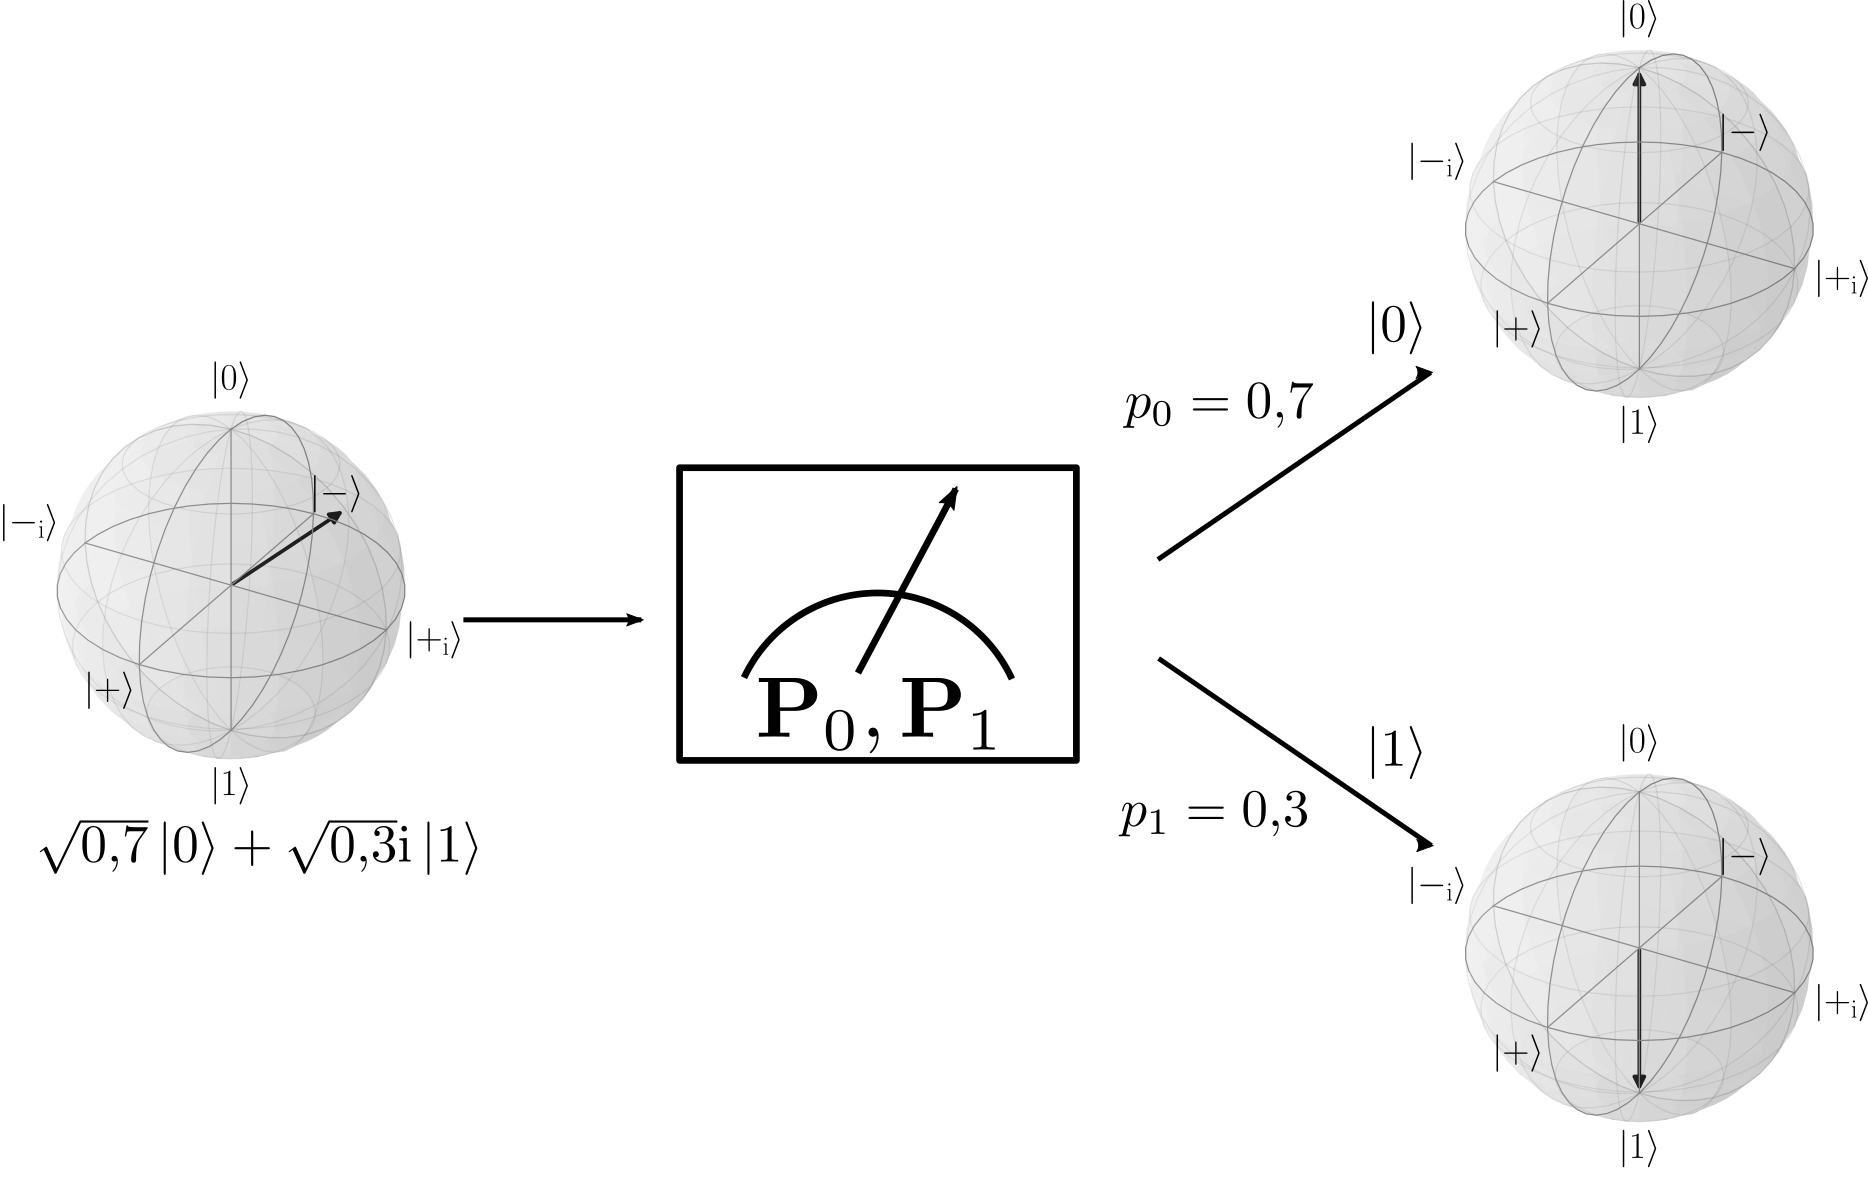
\includegraphics[height=0.38\textheight]{pics/pomiar_sz}}\\
	\subbottom[Pomiar z~wykorzystaniem macierzy $\mat{Q}_{-_\i}=\ketbra{-_\i}{-_\i}, \mat{Q}_{+_\i}=\ketbra{+_\i}{+_\i}$.\label{rys:pomiar-Q}]%
	{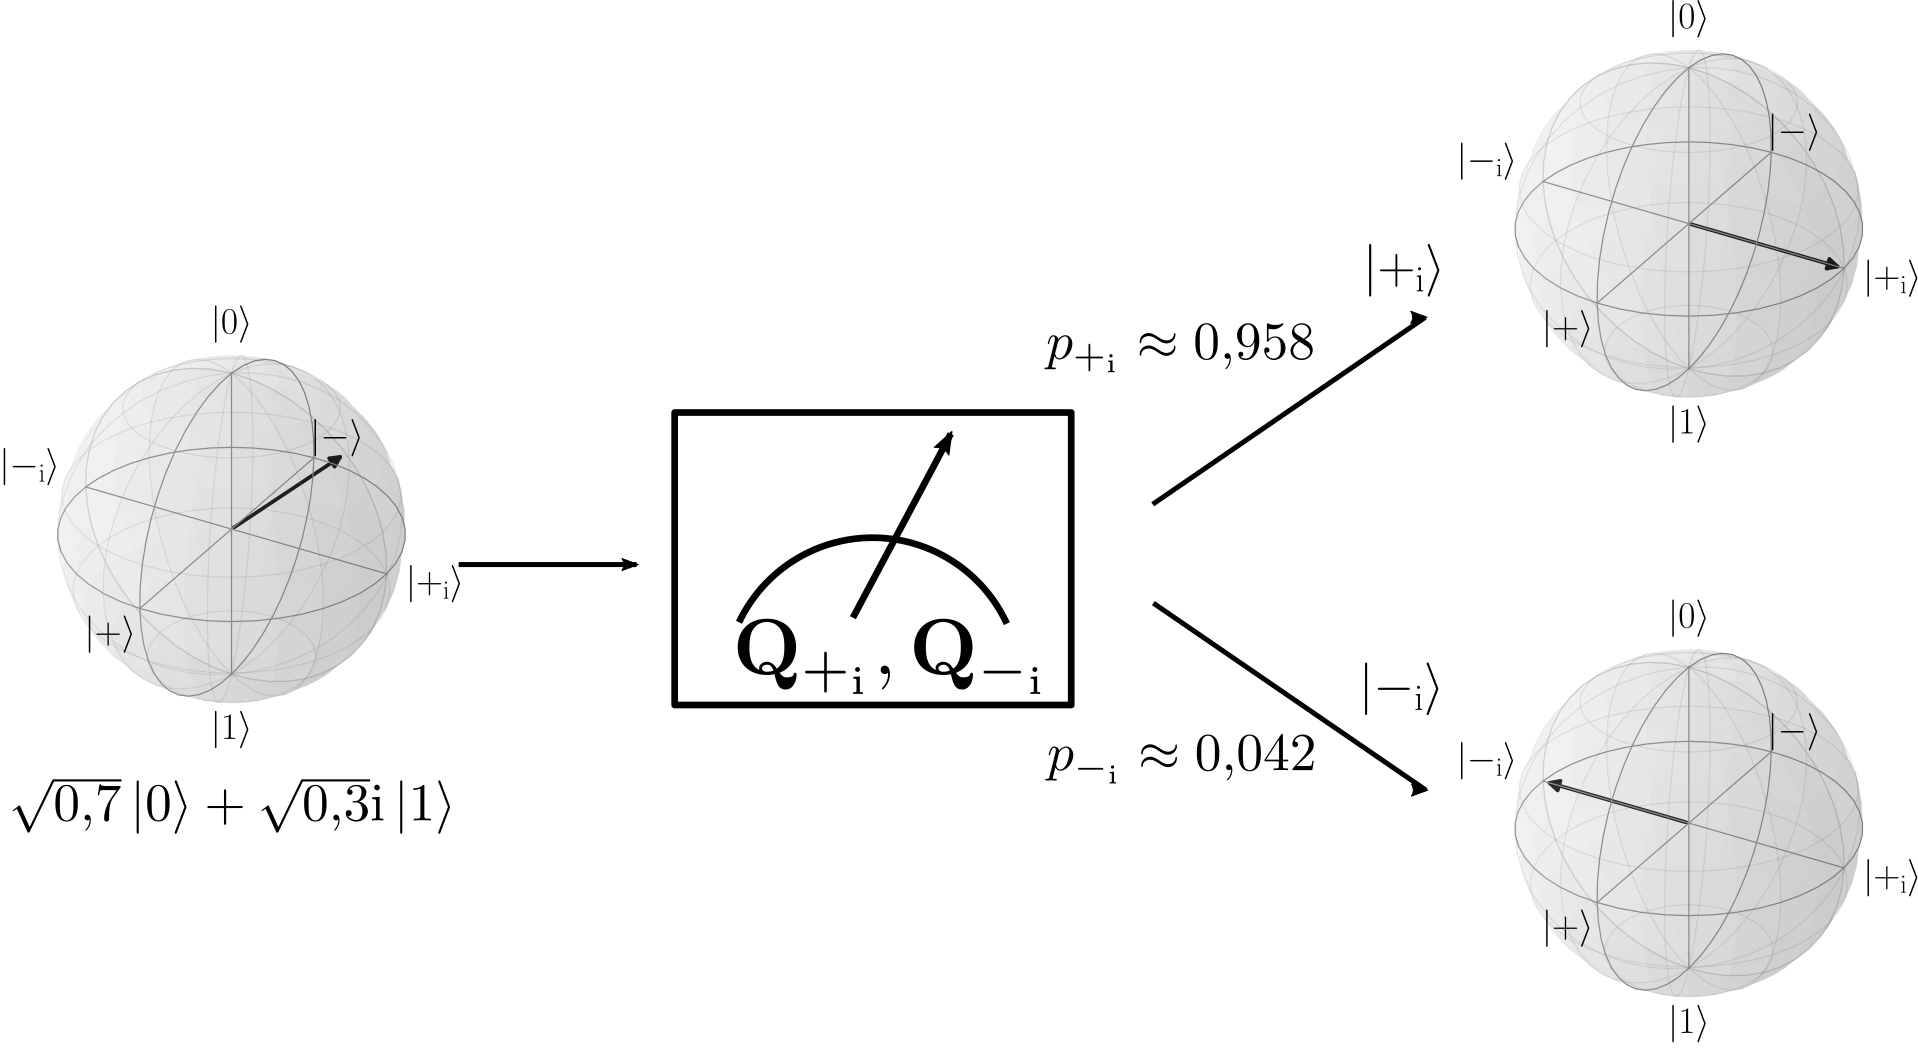
\includegraphics[height=0.38\textheight]{pics/pomiar_sy}}
	\caption{Schemat dwóch różnych pomiarów kwantowych tego samego stanu
		$\sqrt{0{,}7}\ket{0}+\sqrt{0{,}3}\i\ket{1}$. W~zależności od~rodzaju pomiaru
		uzyskujemy inne wyniki z~różnymi prawdopodobieństwami oraz~inne stany
		po~wykonaniu pomiaru.
		Takie zachowanie układów jest charakterystyczne dla~mechaniki kwantowej.
	}
	\label{rys:pomiar}
\end{figure}


\subsection{Szeregowanie pomiarów}
Tak~samo jak~bramki kwantowe, pomiary mogą być wykonywane jeden po~drugim.\index{pomiar!szeregowanie}
Oczywiście trzeba brać pod~uwagę, że~pierwszy pomiar zmieni stan kwantowy
i~wynik drugiego pomiaru będzie zależał od~wyniku pierwszego pomiaru.

Jeżeli~wykonujemy ten sam pomiar wielokrotnie, to wynik, który otrzymaliśmy
z~pierwszego pomiaru, otrzymamy też w~każdym następnym pomiarze. Weźmy zatem
pod~uwagę stan $\ket{\psi}$
oraz~pomiar
$$\mathcal{P}=\{\mat{P}_0,\mat{P}_1, \ldots, \mat{P}_{n-1}\}.$$
Jeżeli~dokonamy
pomiaru tego stanu jednokrotnie i~zmierzymy wynik $i$, to otrzymamy stan
$$
	\ket{\psi_i} = \frac{\mat{P}_i\ket{\psi}}{\norm{\mat{P}_i\ket{\psi}}}.
$$
Zmierzmy ten stan jeszcze raz i~zobaczmy, jakie jest prawdopodobieństwo zmierzenia wyniku $j$:
$$
	p_j'=\norm{\mat{P}_j\ket{\psi_i}}^2 = \norm{\frac{\mat{P}_j\mat{P}_i\ket{\psi}}{\norm{\mat{P}_i\ket{\psi}}}}^2.
$$
Ponieważ $\mat{P}_j \mat{P}_i$ jest równe $\mat{0}$ dla~różnych $i$ i~$j$, to prawdopodobieństwo
otrzymania za~drugim razem wyniku innego niż~za~pierwszym wynosi 0.
Natomiast prawdopodobieństwo otrzymania za~drugim razem tego samego wyniku co~za~pierwszym razem wynosi
$$
	p_i'=\norm{\frac{\mat{P}_i\mat{P}_i\ket{\psi}}{\norm{\mat{P}_i\ket{\psi}}}}^2 = \norm{\frac{\mat{P}_i\ket{\psi}}{\norm{\mat{P}_i\ket{\psi}}}}^2 =
	\frac{1}{\norm{\mat{P}_i\ket{\psi}}^2} \norm{\mat{P}_i\ket{\psi}}^2 = 1.
$$
Zatem widać, że~jeżeli~za~pierwszym razem wykonaliśmy pomiar
$\mathcal{P}$ na~stanie $\ket{\psi}$ i~otrzymaliśmy wynik~$i$ oraz~stan
po~pomiarze $\ket{\psi_i}$, to po~wykonaniu tego samego pomiaru raz
jeszcze na~otrzymanym stanie uzyskamy ten sam wynik~$i$. Zatem stan
$\ket{\psi_i}$ pozostanie niezmieniony.

\subsection{Pomiar częściowy stanu wielosystemowego}
Zobaczmy teraz, co się~dzieje, gdy~wykonamy pomiar częściowy stanu pierwszego
kubitu na~stanie złożonym z~dwóch kubitów. Przez \newterm{pomiar
	częściowy}\index{pomiar!częściowy} rozumiemy taki pomiar wykonywany na~układzie
wielu kubitów, że~na~części z~nich dokonujemy pomiaru trywialnego, a~na~części --
nietrywialnego.

Załóżmy, że~mamy do~dyspozycji stan
$$
	\ket{\psi} = \alpha_{00}\ket{00} + \alpha_{01}\ket{01} + \alpha_{10}\ket{10} + \alpha_{11}\ket{11}
$$
i~wykonujemy pomiar $\mathcal{P}=\{\mat{P}_0=\ketbra{0}{0},\mat{P}_1=\ketbra{1}{1}\}$
na~pierwszym kubicie oraz pomiar trywialny na drugim.
Wówczas wynik $0$ z~pomiaru pierwszego kubitu uzyskujemy z~prawdopodobieństwem
\begin{align*}
	p_{0?} & = \norm{\mat{P}_0\otimes\mat{\id}_? \ket{\psi}}^2 =
	\norm{\begin{bmatrix} 1 & 0 & 0 & 0 \\  0 & 1 & 0 & 0 \\  0 & 0 & 0 & 0 \\  0 & 0 & 0 & 0 \end{bmatrix}
		\begin{bmatrix} \alpha_{00} \\ \alpha_{01} \\ \alpha_{10} \\ \alpha_{11} \end{bmatrix}}^2 =
	\norm{\begin{bmatrix} \alpha_{00} \\ \alpha_{01} \\ 0 \\ 0 \end{bmatrix}}^2  =                       \\
	       & = \abs{\alpha_{00}}^2 + \abs{\alpha_{01}}^2.
\end{align*}
Odpowiednio wynik $1$ uzyskujemy z~prawdopodobieństwem $$p_{1?} = \abs{\alpha_{10}}^2 + \abs{\alpha_{11}}^2.$$
Stan po~zmierzeniu $0$ na~pierwszym kubicie staje~się
$$
	\ket{\psi_{0?}}=
	\frac{\alpha_{00}\ket{00} + \alpha_{01}\ket{01}}{\sqrt{|\alpha_{00}|^2 + |\alpha_{01}|^2}} =
	\ket{0}\otimes\frac{\alpha_{00}\ket{0} + \alpha_{01}\ket{0}}{\sqrt{|\alpha_{00}|^2 + |\alpha_{01}|^2}},
$$
a po~zmierzeniu $1$ -- staje~się
$$
	\ket{\psi_{1?}}=
	\frac{\alpha_{10}\ket{10} + \alpha_{11}\ket{11}}{\sqrt{|\alpha_{10}|^2 + |\alpha_{11}|^2}} =
	\ket{1}\otimes\frac{\alpha_{10}\ket{0} + \alpha_{11}\ket{1}}{\sqrt{|\alpha_{10}|^2 + |\alpha_{11}|^2}}.
$$

Zobaczmy, co się~stanie, gdy przeprowadzimy go na~stanie Bella
$\ket{\Phi^+}=\frac{1}{\sqrt{2}}(\ket{00}+\ket{11})$. Wówczas mamy
$\alpha_{00}=\alpha_{11}=\frac{1}{\sqrt{2}}$ oraz $\alpha_{01}=\alpha_{10}=0$. Zatem zmierzenie $0$
na~pierwszym kubicie da nam stan po~pomiarze $\ket{00}$, a~zmierzenie $1$ da nam
stan $\ket{11}$. Czyli~-- jak widać -- wynik pomiaru na~pierwszym kubicie determinuje
stan po~pomiarze drugiego kubitu, a~zatem również wynik pomiaru na~drugim. Efekt
taki jest utożsamiany ze~splątaniem kwantowym i~-- jako taki -- jest on bardzo istotny dla~informatyki kwantowej.

\section{Podsumowanie}
W~powyższym rozdziale wprowadziliśmy pojęcia stanu, bramki kwantowej i~pomiaru kwantowego. Dzięki temu wiemy teraz,
jak opisywane są układy kwantowe, jak zmieniają~się w~czasie i~jak są
odczytywane ich właściwości. W~komputerach i~systemach kwantowych te operacje wykonywane są
cyklicznie po~to, by~implementować protokoły lub~algorytmy kwantowe.

